%%%%%%%%%%
% if Appendix is needed:
%%%%%%%%%%
\renewcommand{\theHchapter}{A\arabic{chapter}}
\appendix
%	\begin{appendices}
\phantomsection

\chapter{Model Measurements}
\label{app:model_measurements}
  \begin{table}
    \centering
    \begin{tabular}{lrl}
    Name & Dimension & Unit [in] \\
    fuselage & Length & $18$\\
            & Diameter &  $3$\\
            & Fin     & $2 \frac{5}{16}$\\
            \\
    Nose-1  & Base & $3$ \\
            & Edge Length & $3 \frac{11}{16}$ \\
            \\
    Nose-2  & Base & $3$ \\
            & Edge Length & $5 \frac{13}{16}$ \\
            \\
    Nose-3  & Base & $3$ \\
            & Edge Length & $8 \frac{11}{16}$ \\
            \\
    Nose-4  & Base & $3$ \\
            & Diameter 1 & $2.91339$ \\
            & Diameter 2 & $2.56$ \\
            & Diameter 3 & $1.57$ \\
            \\
    Nose-5  & Base & $3$ \\
            & Diameter 1 & $2.87$ \\
            & Diameter 2 & $2.52$ \\
            & Diameter 3 & $1.89$ \\
            & Diameter 3 & $0.83$ \\
    \end{tabular}
    \caption{Model dimensions}
    \label{tab:models}
  \end{table}

\chapter{Models}
\label{app:models}

  \begin{figure}[htbp]
    \centering
    \begin{subfigure}{.5\textwidth}
      \centering
      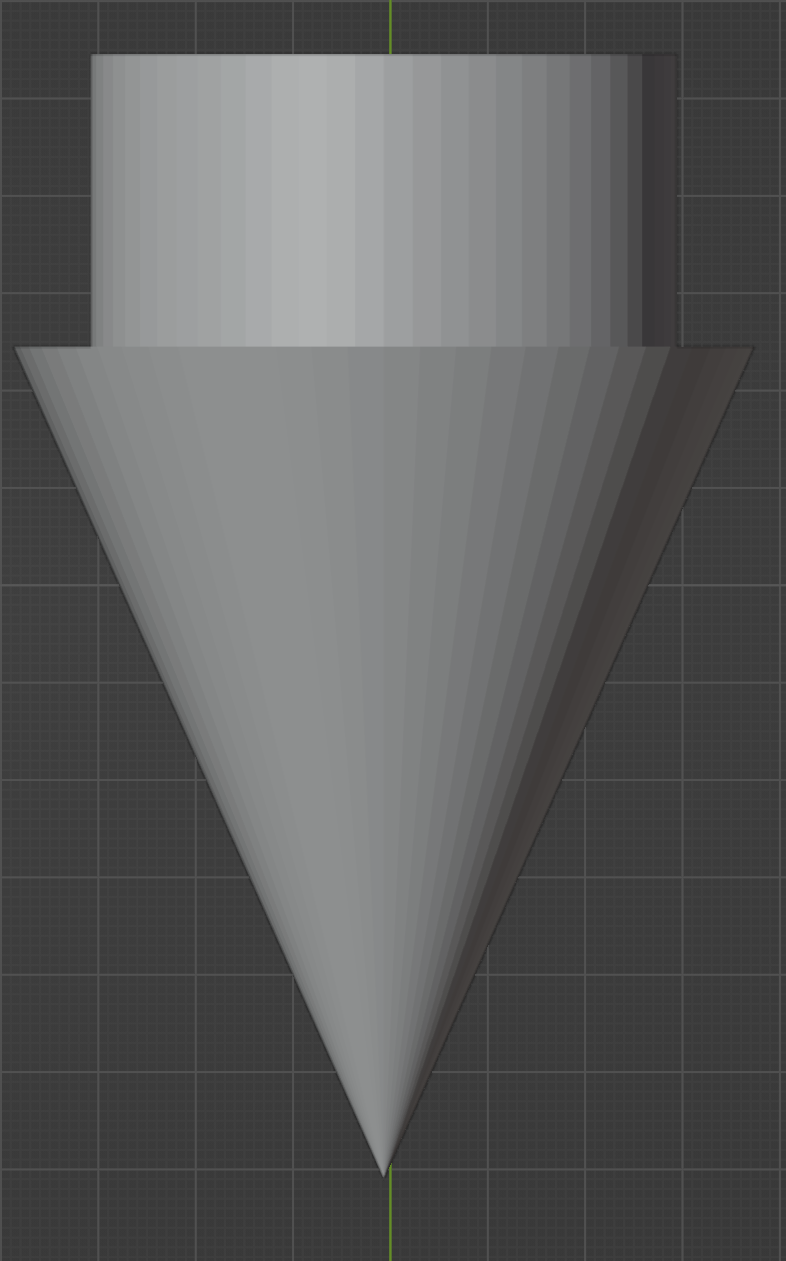
\includegraphics[width=.8\linewidth]{nose_1.png}
    \end{subfigure}%
    \begin{subfigure}{.5\textwidth}
      \centering
      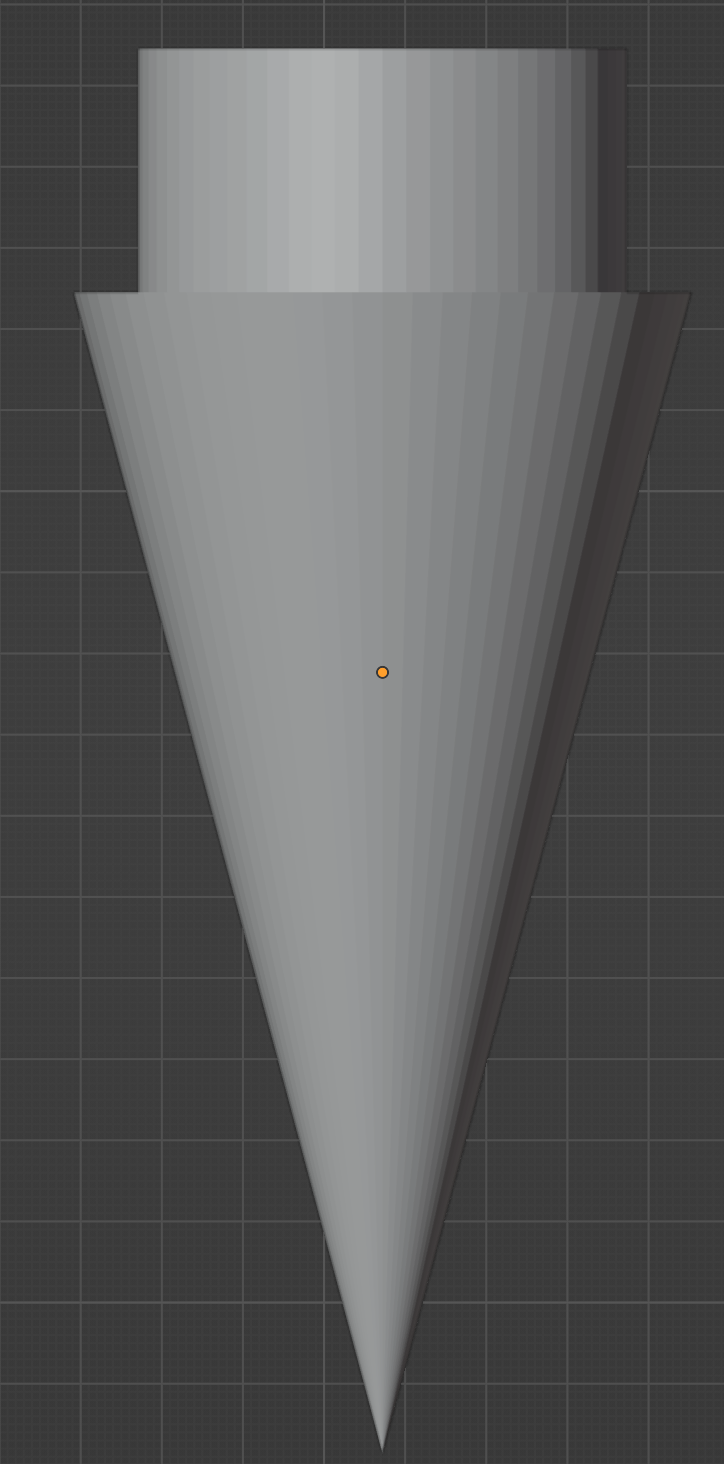
\includegraphics[width=.8\linewidth]{nose_2.png}
    \end{subfigure}
    \caption{Simulation targets 1 and 2}
    \label{fig:nose_1_2}
  \end{figure}

  \begin{figure}[htbp]
    \centering
    \begin{subfigure}{.5\textwidth}
      \centering
      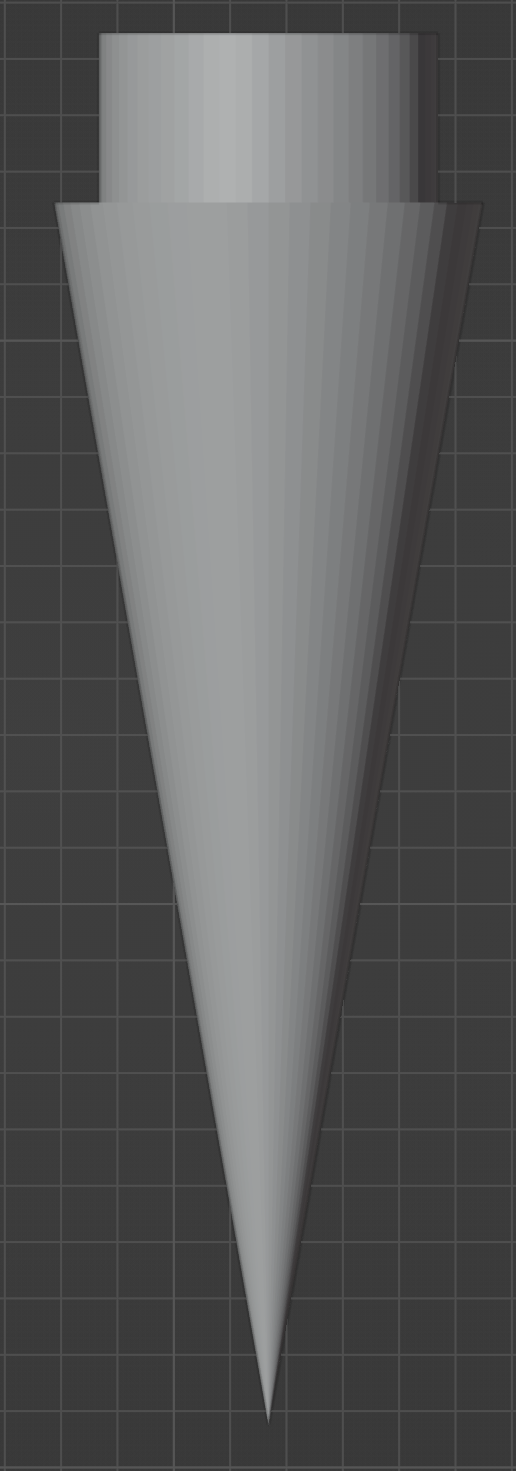
\includegraphics[width=.8\linewidth]{nose_3.png}
    \end{subfigure}%
    \begin{subfigure}{.5\textwidth}
      \centering
      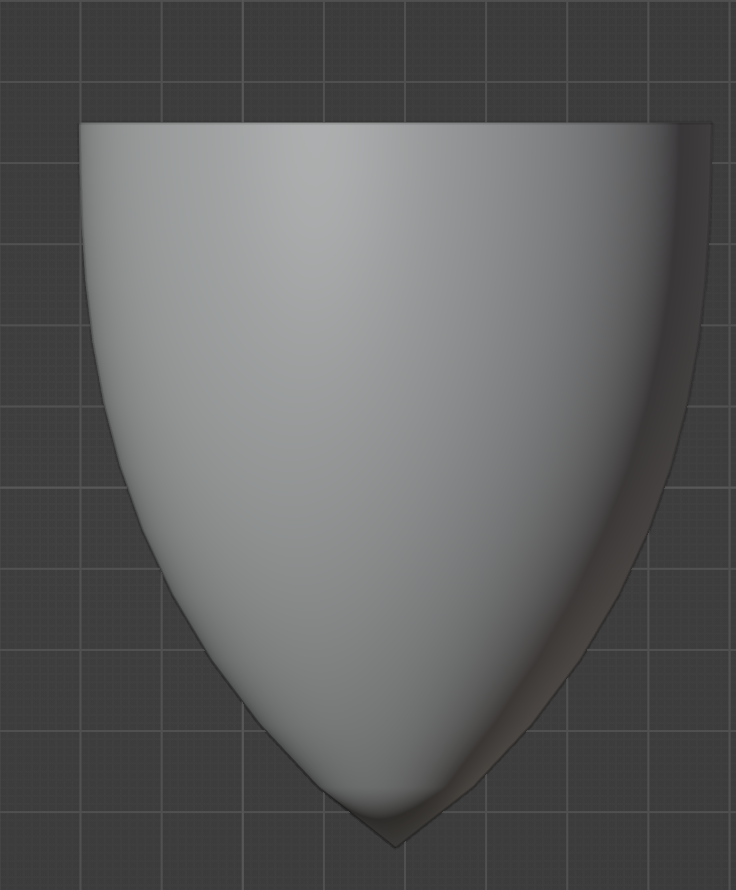
\includegraphics[width=.8\linewidth]{nose_4.png}
    \end{subfigure}
    \caption{Simulation targets 3 and 4}
    \label{fig:nose_3_4}
  \end{figure}

  \begin{figure}[htbp]
    \centering
    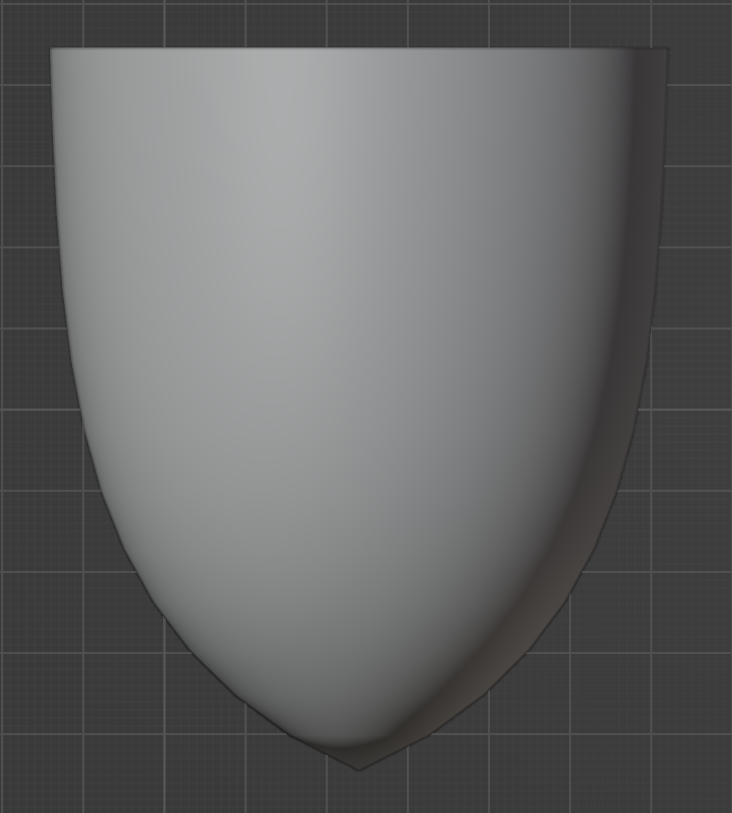
\includegraphics[width=.8\linewidth]{nose_5.png}
    \caption{Simulation targets 3 and 4}
    \label{fig:nose_5}
  \end{figure}


\chapter{Measurement Results}
\label{app:measurement_results}
  \begin{figure}[htbp]
    \centering
    \begin{subfigure}{.5\textwidth}
      \centering
      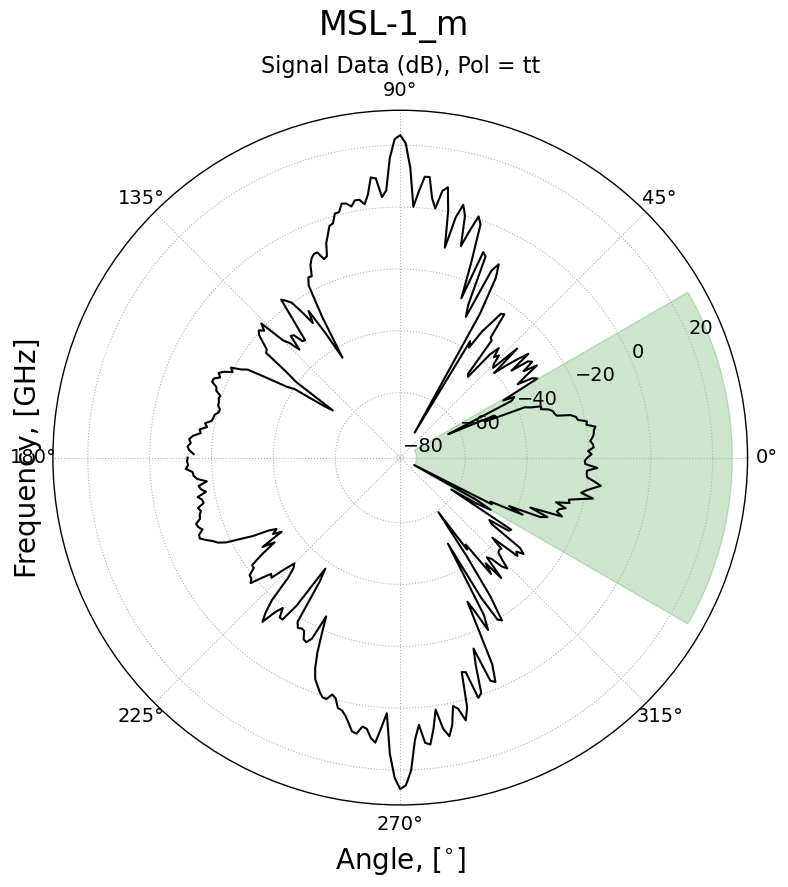
\includegraphics[width=.8\linewidth]{MSL-1_m_dB_tt_5GHz.png}
    \end{subfigure}%
    \begin{subfigure}{.5\textwidth}
      \centering
      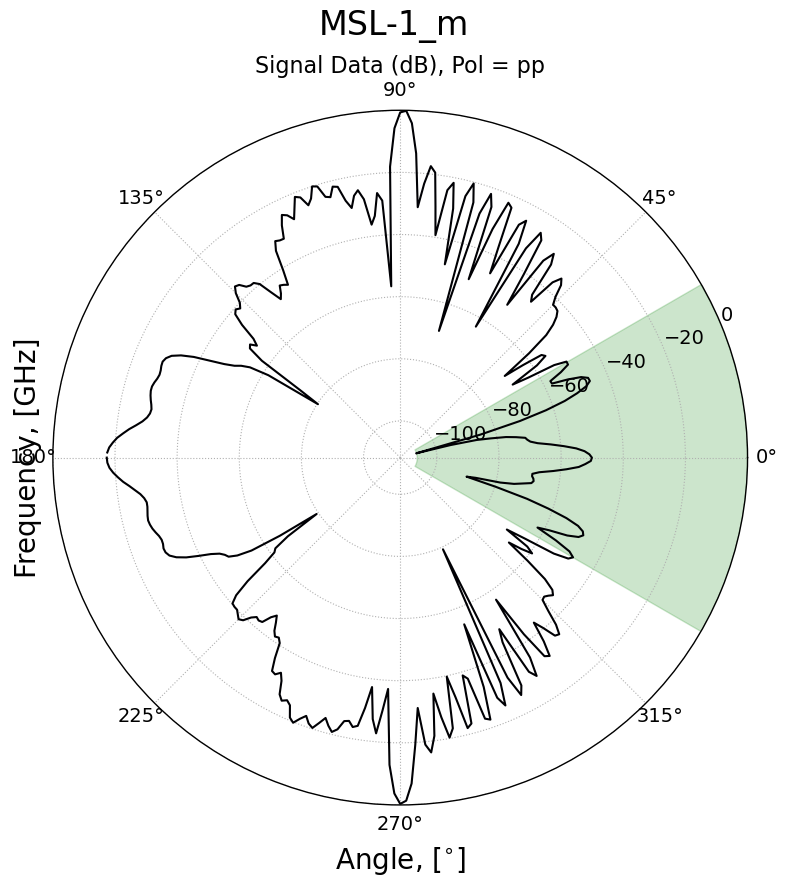
\includegraphics[width=.8\linewidth]{MSL-1_m_dB_pp_5GHz.png}
    \end{subfigure}
    \caption{Missile 1 \textcolor{green}{(Test)}:  RCS cut at 5 GHz. Vertical (tt) and Horizontal (pp) polarizations }
    \label{fig:n1}
  \end{figure}

  \begin{figure}[htbp]
    \centering
    \begin{subfigure}{.5\textwidth}
      \centering
      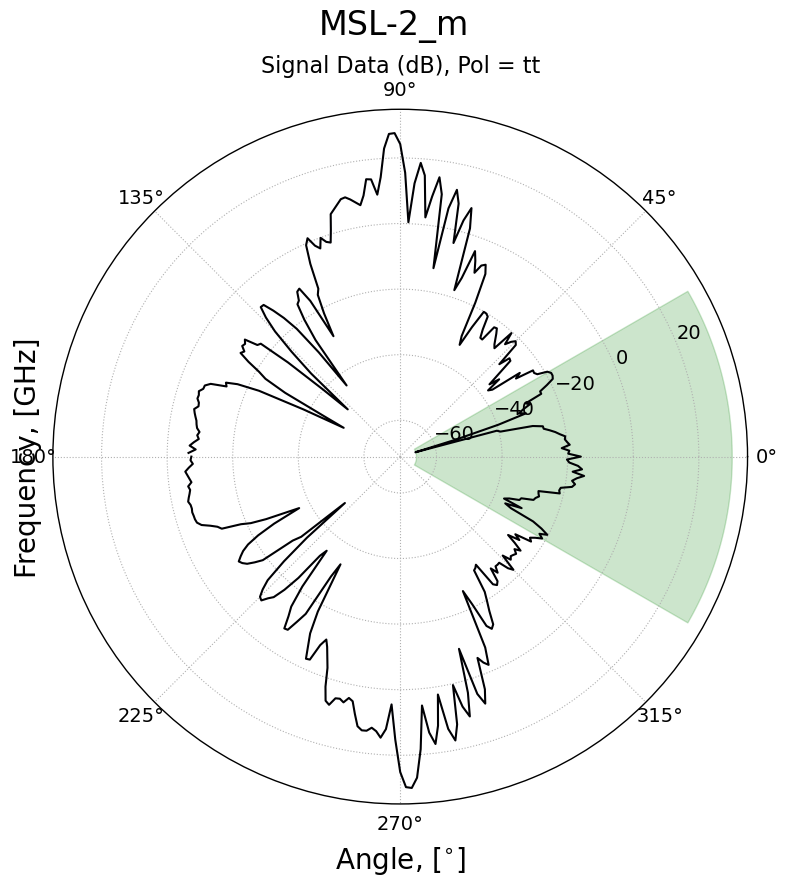
\includegraphics[width=.8\linewidth]{MSL-2_m_dB_tt_5GHz.png}
    \end{subfigure}%
    \begin{subfigure}{.5\textwidth}
      \centering
      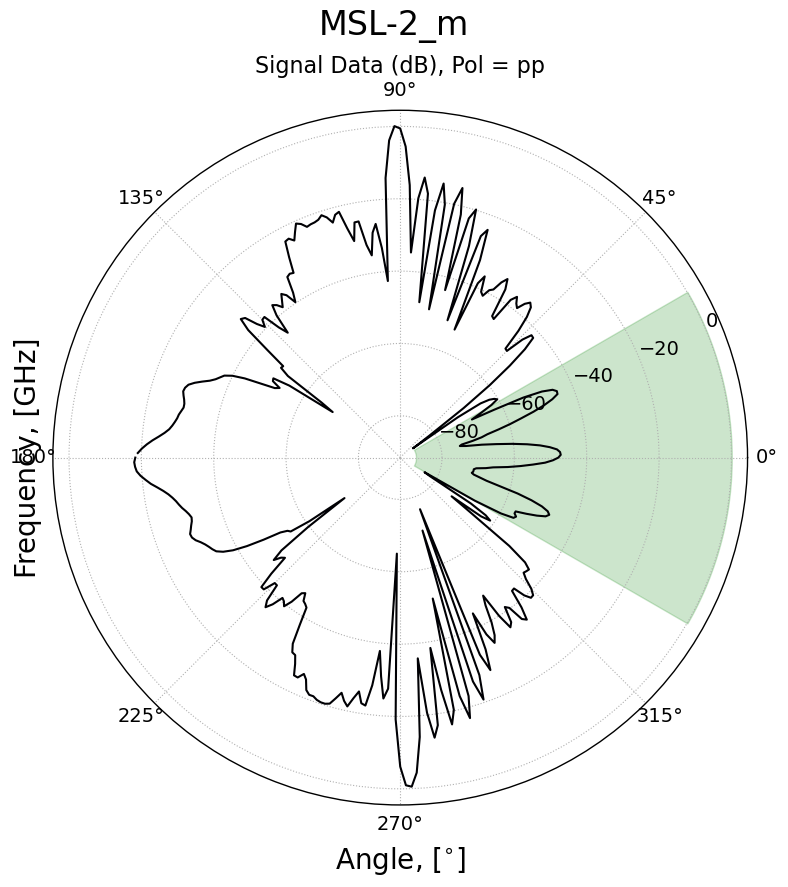
\includegraphics[width=.8\linewidth]{MSL-2_m_dB_pp_5GHz.png}
    \end{subfigure}
    \caption{Missile 2 \textcolor{green}{(Test)}:  RCS cut at 5 GHz. Vertical (tt) and Horizontal (pp) polarizations }
    \label{fig:n2}
  \end{figure}

  \begin{figure}[htbp]
    \centering
    \begin{subfigure}{.5\textwidth}
      \centering
      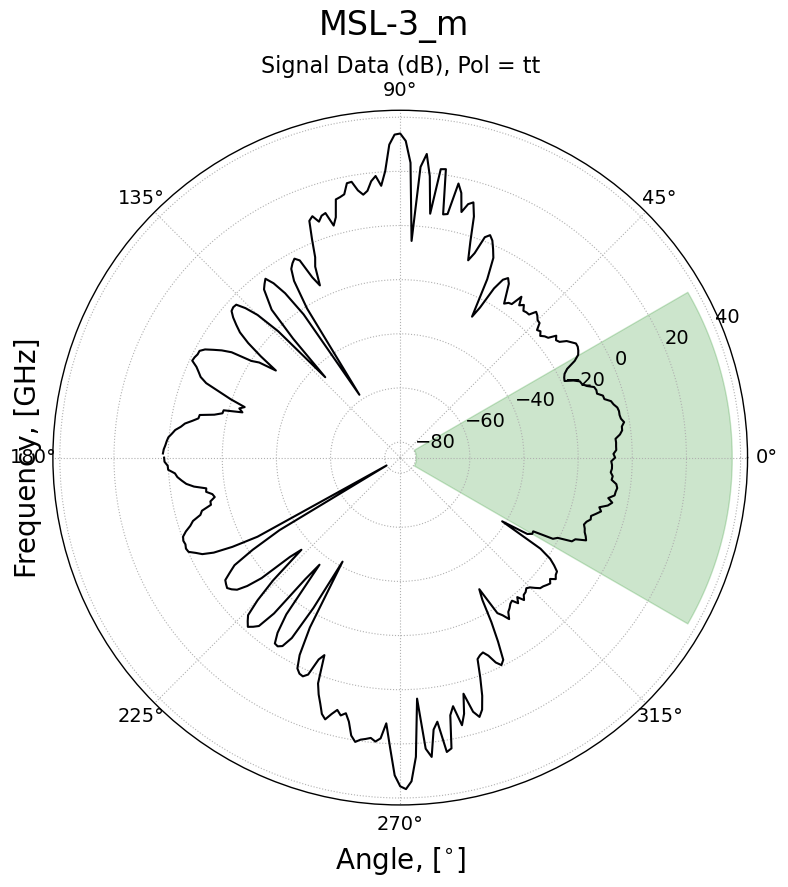
\includegraphics[width=.8\linewidth]{MSL-3_m_dB_tt_5GHz.png}
    \end{subfigure}%
    \begin{subfigure}{.5\textwidth}
      \centering
      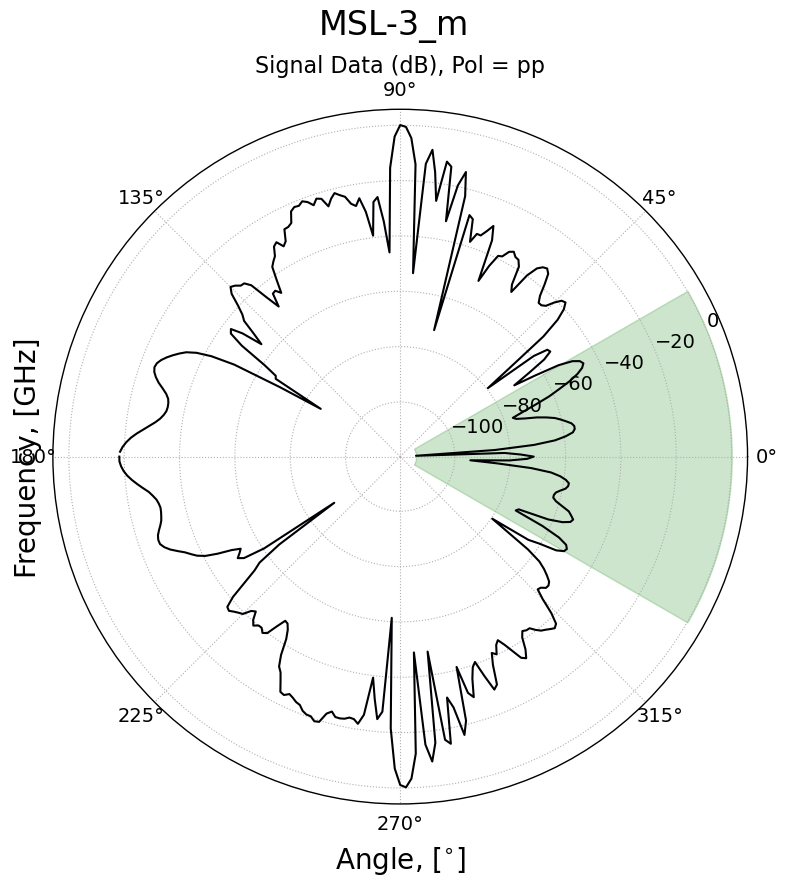
\includegraphics[width=.8\linewidth]{MSL-3_m_dB_pp_5GHz.png}
    \end{subfigure}
    \caption{Missile 3 \textcolor{green}{(Test)}:  RCS cut at 5 GHz. Vertical (tt) and Horizontal (pp) polarizations }
    \label{fig:n3}
  \end{figure}

  \begin{figure}[htbp]
    \centering
    \begin{subfigure}{.5\textwidth}
      \centering
      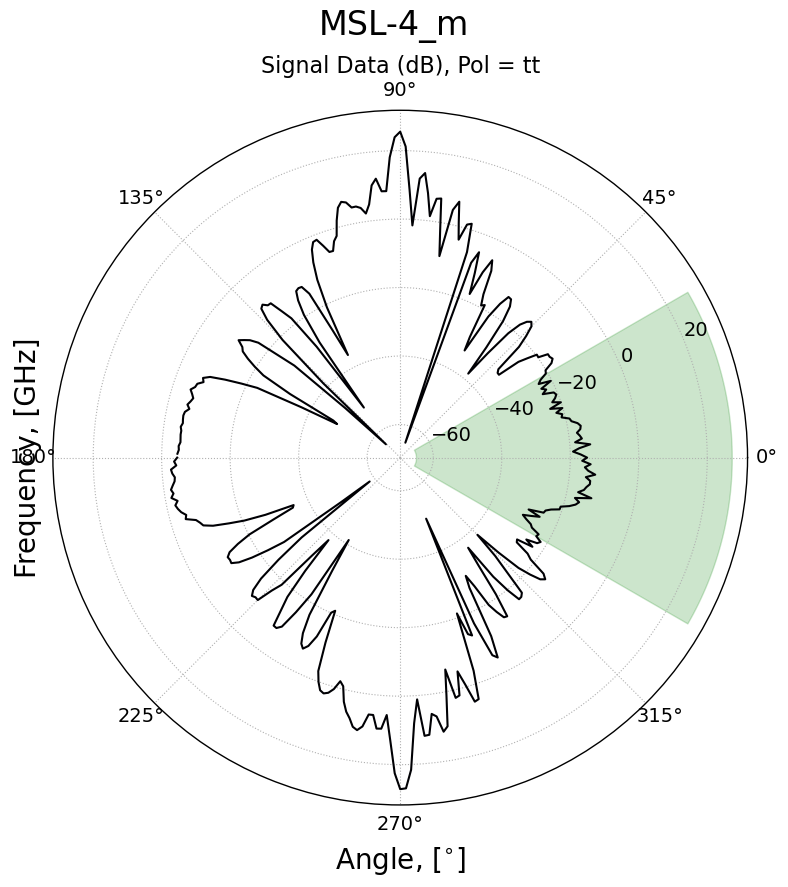
\includegraphics[width=.8\linewidth]{MSL-4_m_dB_tt_5GHz.png}
    \end{subfigure}%
    \begin{subfigure}{.5\textwidth}
      \centering
      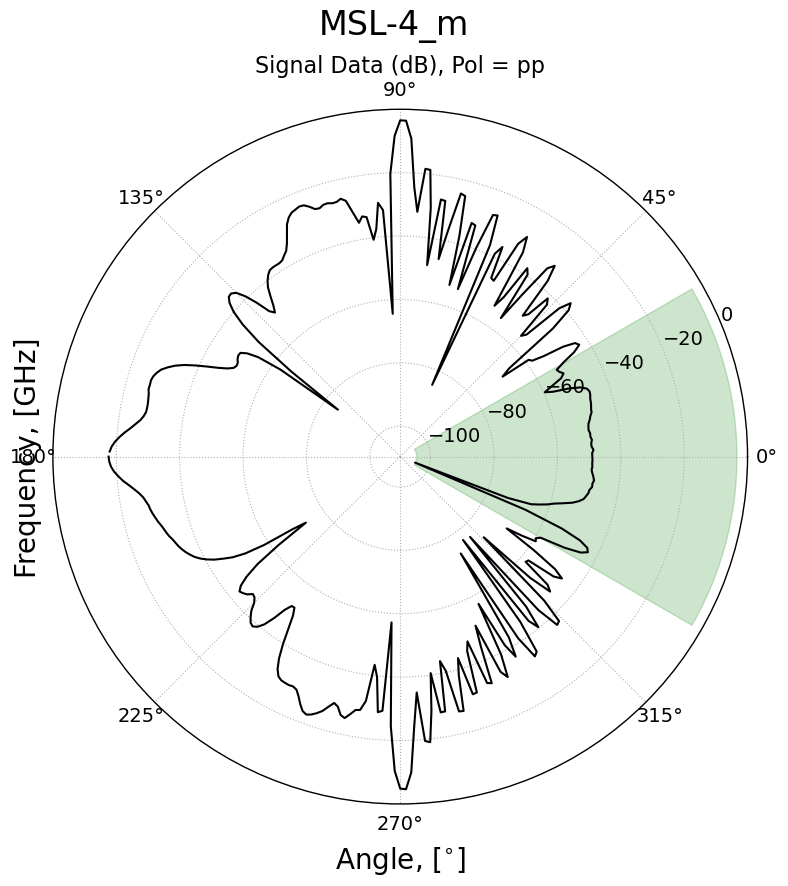
\includegraphics[width=.8\linewidth]{MSL-4_m_dB_pp_5GHz.png}
    \end{subfigure}
    \caption{Missile 4 \textcolor{green}{(Test)}:  RCS cut at 5 GHz. Vertical (tt) and Horizontal (pp) polarizations }
    \label{fig:n4}
  \end{figure}

  \begin{figure}[htbp]
    \centering
    \begin{subfigure}{.5\textwidth}
      \centering
      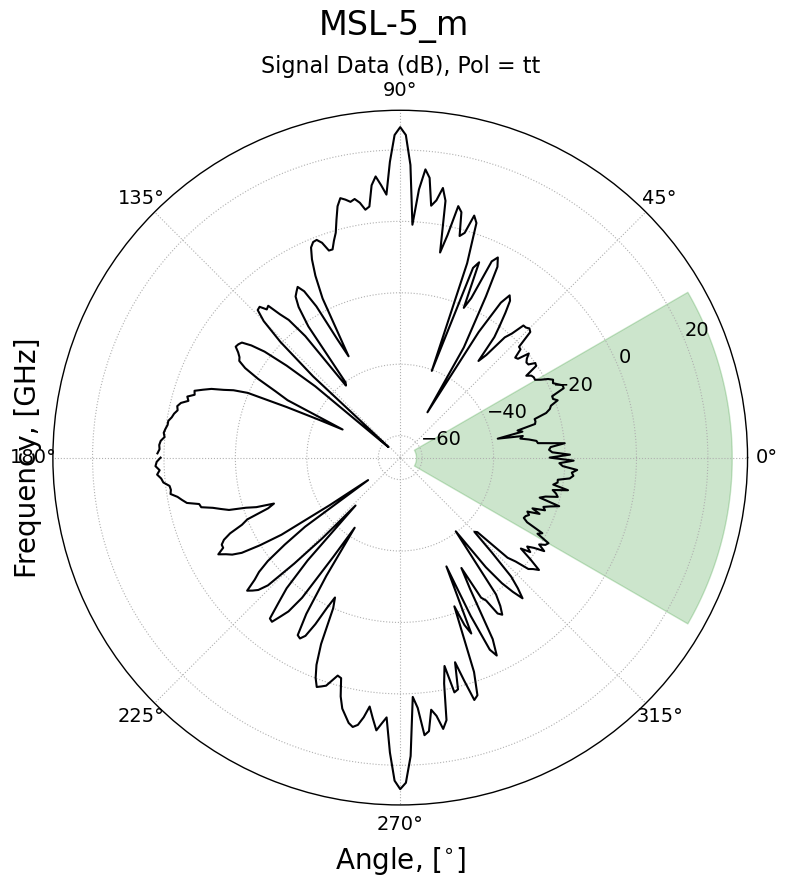
\includegraphics[width=.8\linewidth]{MSL-5_m_dB_tt_5GHz.png}
    \end{subfigure}%
    \begin{subfigure}{.5\textwidth}
      \centering
      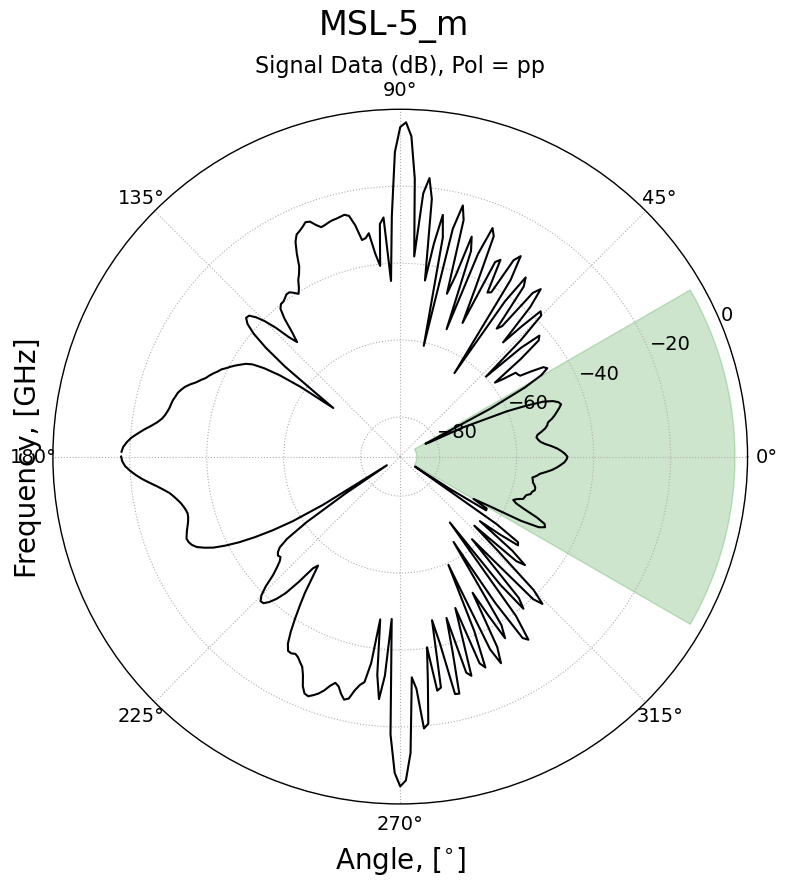
\includegraphics[width=.8\linewidth]{MSL-5_m_dB_pp_5GHz.png}
    \end{subfigure}
    \caption{Missile 5 \textcolor{green}{(Test)}:  RCS cut at 5 GHz. Vertical (tt) and Horizontal (pp) polarizations }
    \label{fig:n5}
  \end{figure}

  \begin{figure}[htbp]
    \centering
    \begin{subfigure}{.5\textwidth}
      \centering
      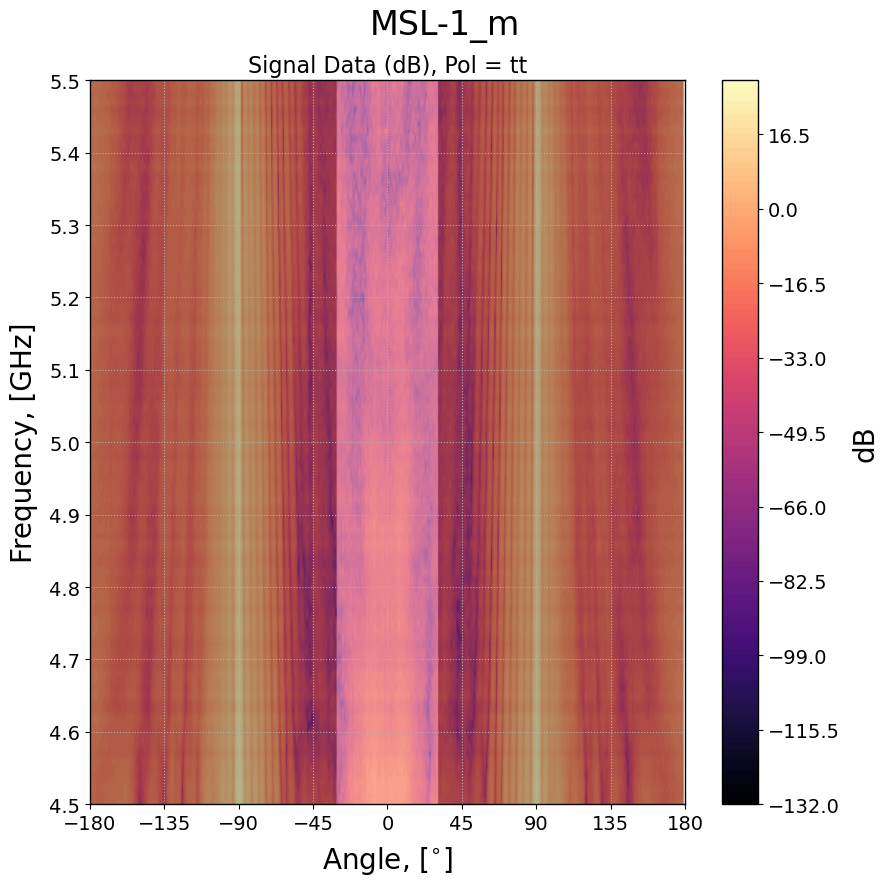
\includegraphics[width=.8\linewidth]{MSL-1_m_dB_tt.png}
    \end{subfigure}%
    \begin{subfigure}{.5\textwidth}
      \centering
      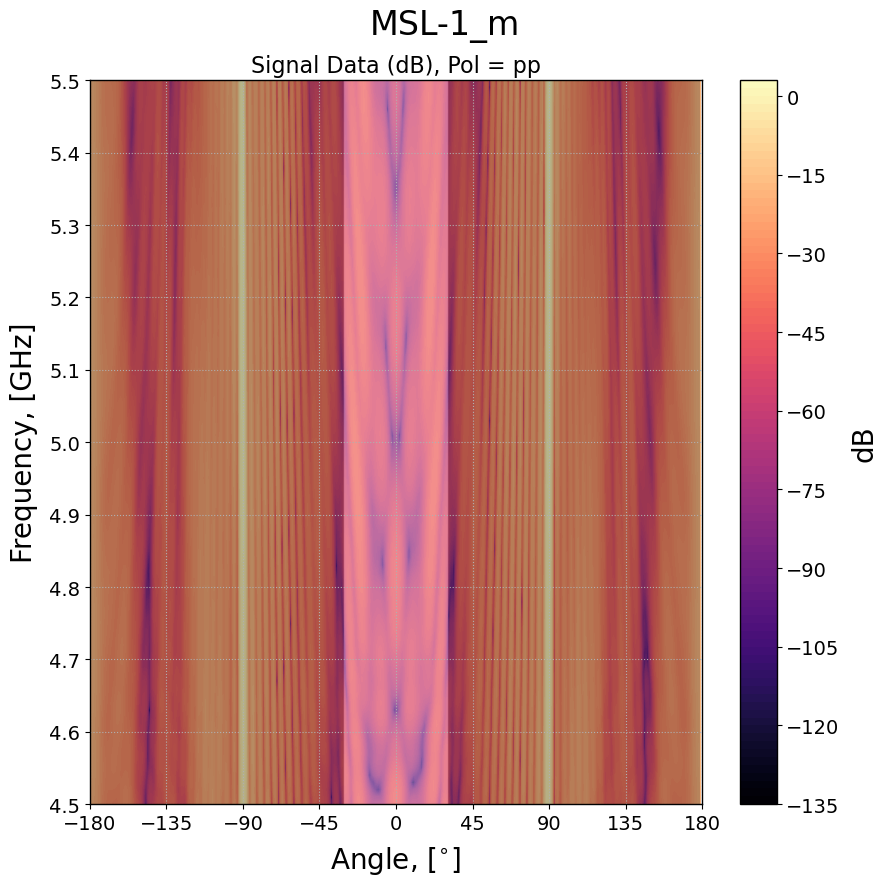
\includegraphics[width=.8\linewidth]{MSL-1_m_dB_pp.png}
    \end{subfigure}
    \caption{Missile 1 \textcolor{green}{(Test)}:  Total RCS. Vertical (tt) and Horizontal (pp) polarizations }
    \label{fig:c1}
  \end{figure}

  \begin{figure}[htbp]
    \centering
    \begin{subfigure}{.5\textwidth}
      \centering
      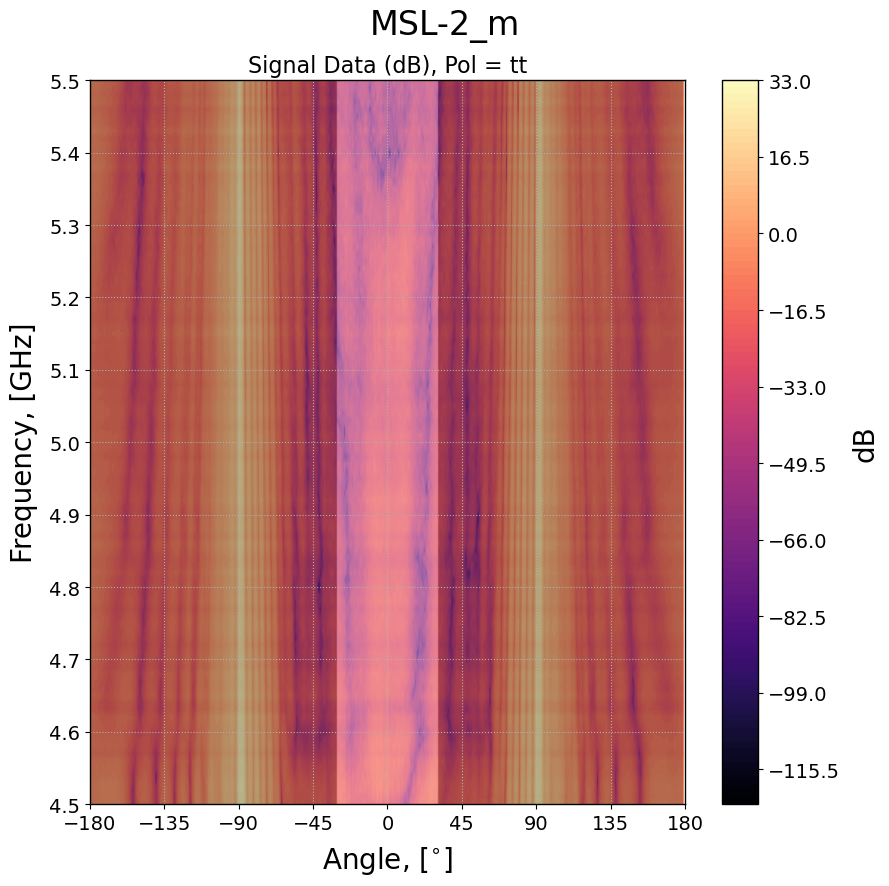
\includegraphics[width=.8\linewidth]{MSL-2_m_dB_tt.png}
    \end{subfigure}%
    \begin{subfigure}{.5\textwidth}
      \centering
      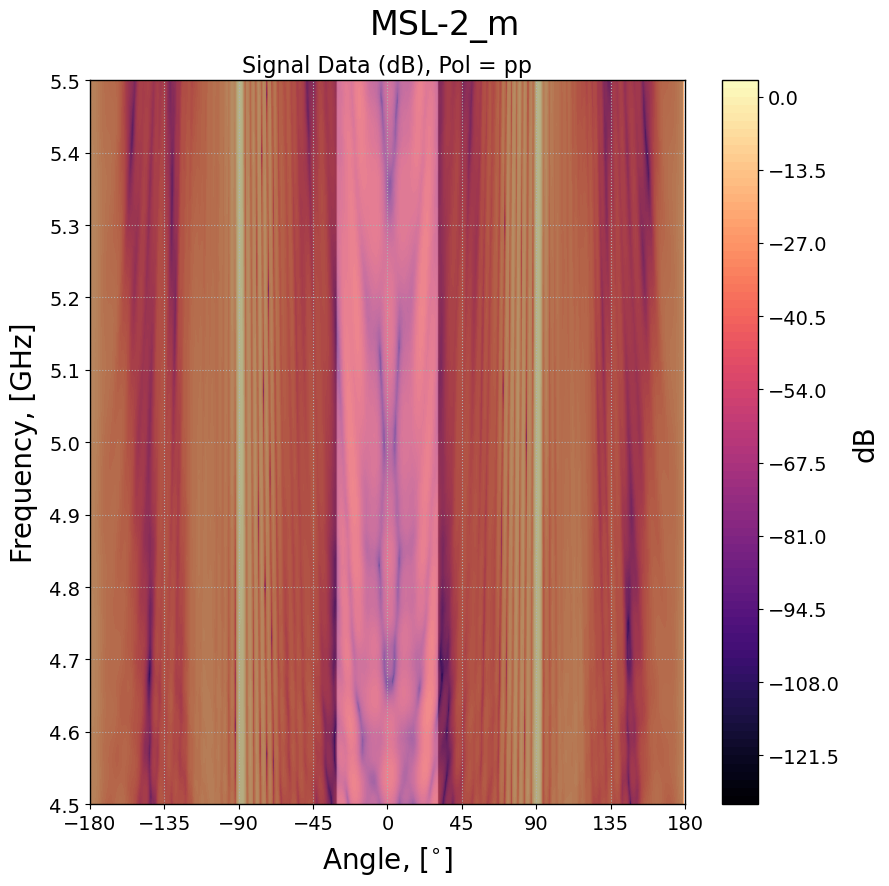
\includegraphics[width=.8\linewidth]{MSL-2_m_dB_pp.png}
    \end{subfigure}
    \caption{Missile 2 \textcolor{green}{(Test)}:  Total RCS. Vertical (tt) and Horizontal (pp) polarizations }
    \label{fig:c2}
  \end{figure}

  \begin{figure}[htbp]
    \centering
    \begin{subfigure}{.5\textwidth}
      \centering
      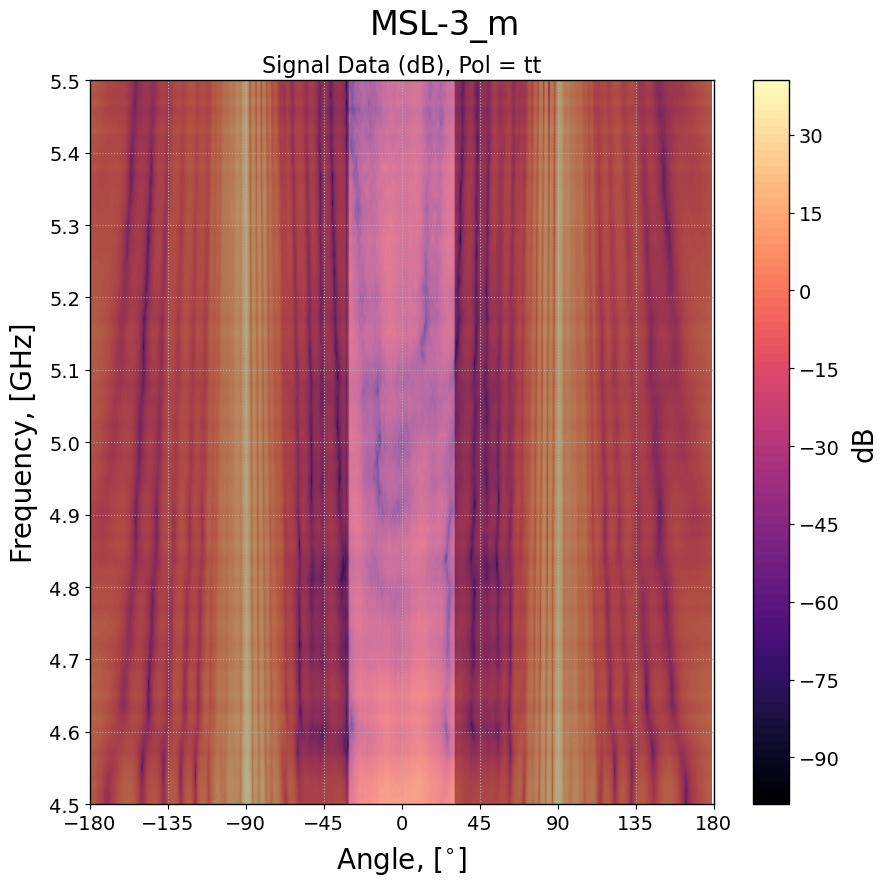
\includegraphics[width=.8\linewidth]{MSL-3_m_dB_tt.png}
    \end{subfigure}%
    \begin{subfigure}{.5\textwidth}
      \centering
      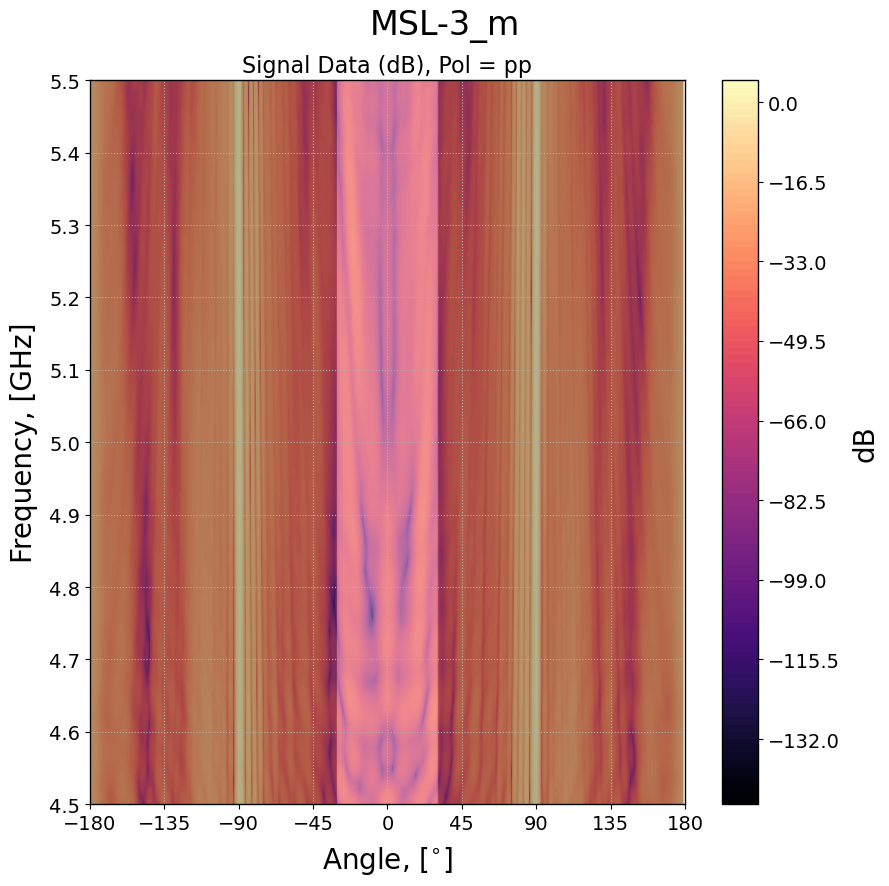
\includegraphics[width=.8\linewidth]{MSL-3_m_dB_pp.png}
    \end{subfigure}
    \caption{Missile 3 \textcolor{green}{(Test)}:  Total RCS. Vertical (tt) and Horizontal (pp) polarizations }
    \label{fig:c3}
  \end{figure}

  \begin{figure}[htbp]
    \centering
    \begin{subfigure}{.5\textwidth}
      \centering
      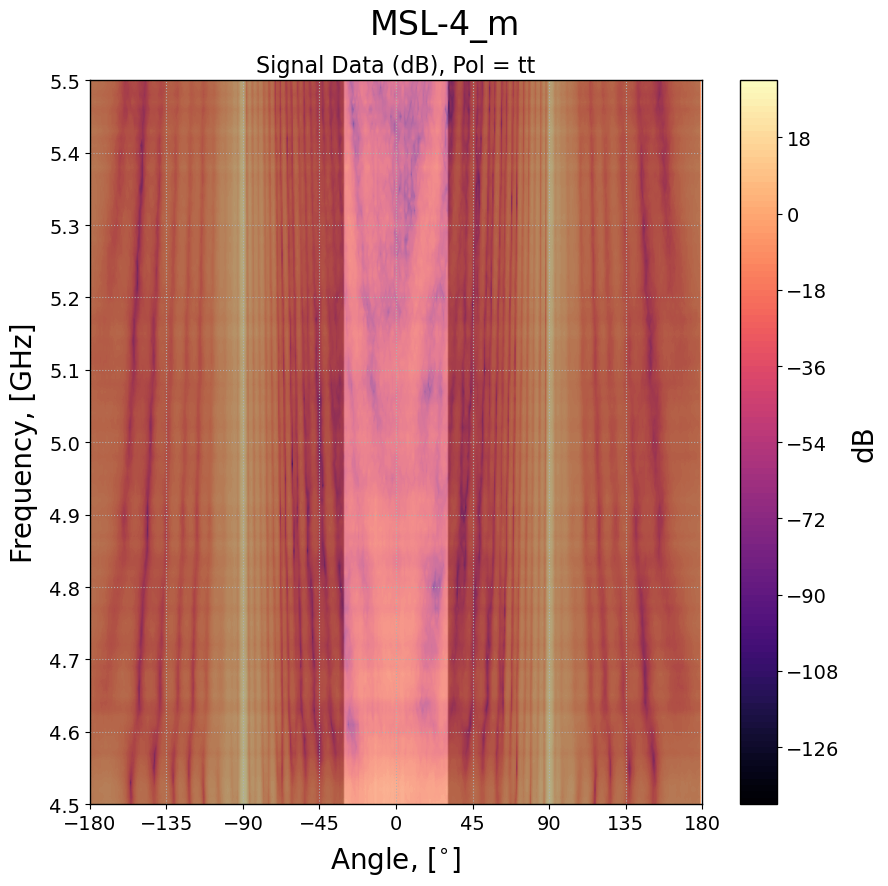
\includegraphics[width=.8\linewidth]{MSL-4_m_dB_tt.png}
    \end{subfigure}%
    \begin{subfigure}{.5\textwidth}
      \centering
      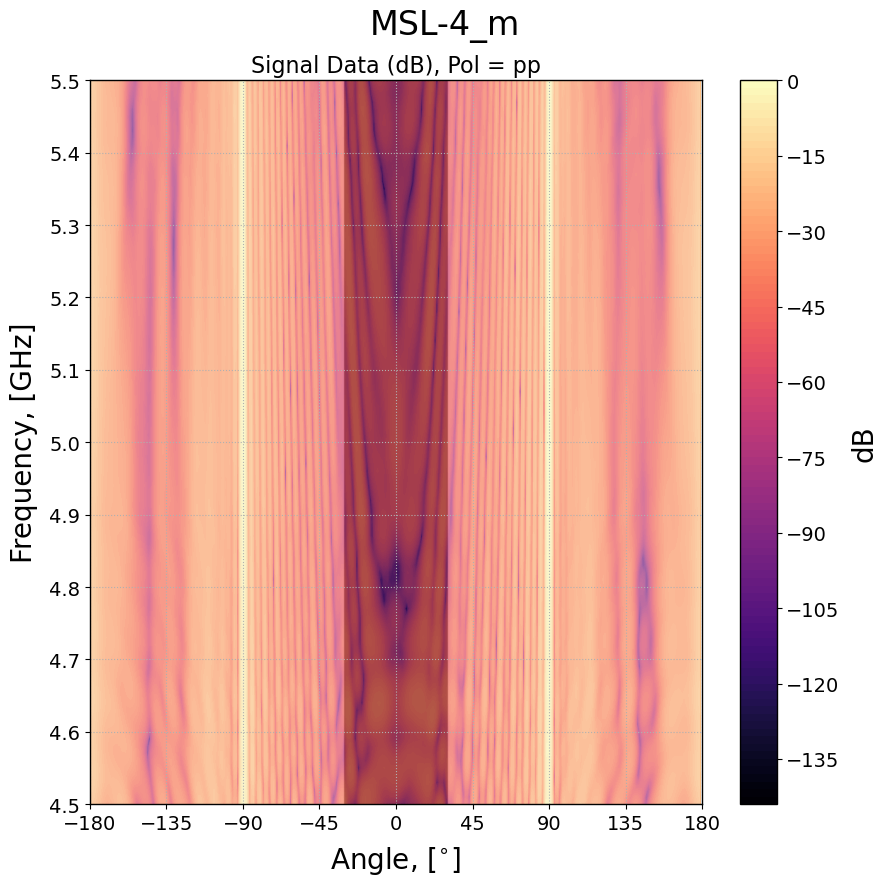
\includegraphics[width=.8\linewidth]{MSL-4_m_dB_pp.png}
    \end{subfigure}
    \caption{Missile 4 \textcolor{green}{(Test)}:  Total RCS. Vertical (tt) and Horizontal (pp) polarizations }
    \label{fig:c4}
  \end{figure}

  \begin{figure}[htbp]
    \centering
    \begin{subfigure}{.5\textwidth}
      \centering
      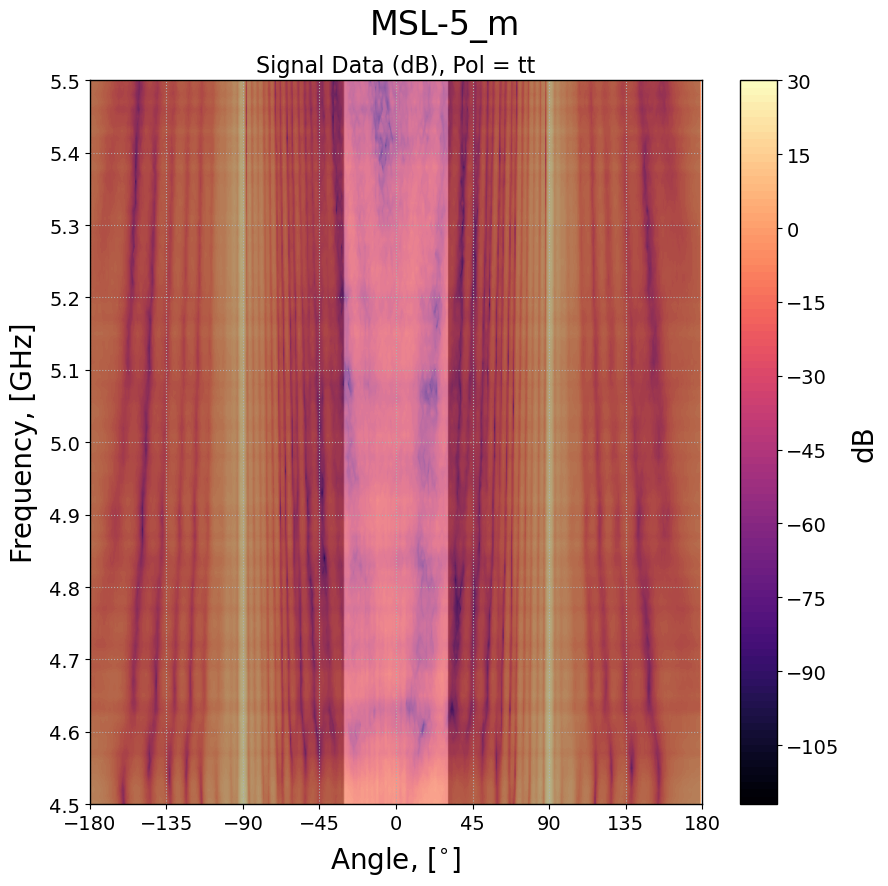
\includegraphics[width=.8\linewidth]{MSL-5_m_dB_tt.png}
    \end{subfigure}%
    \begin{subfigure}{.5\textwidth}
      \centering
      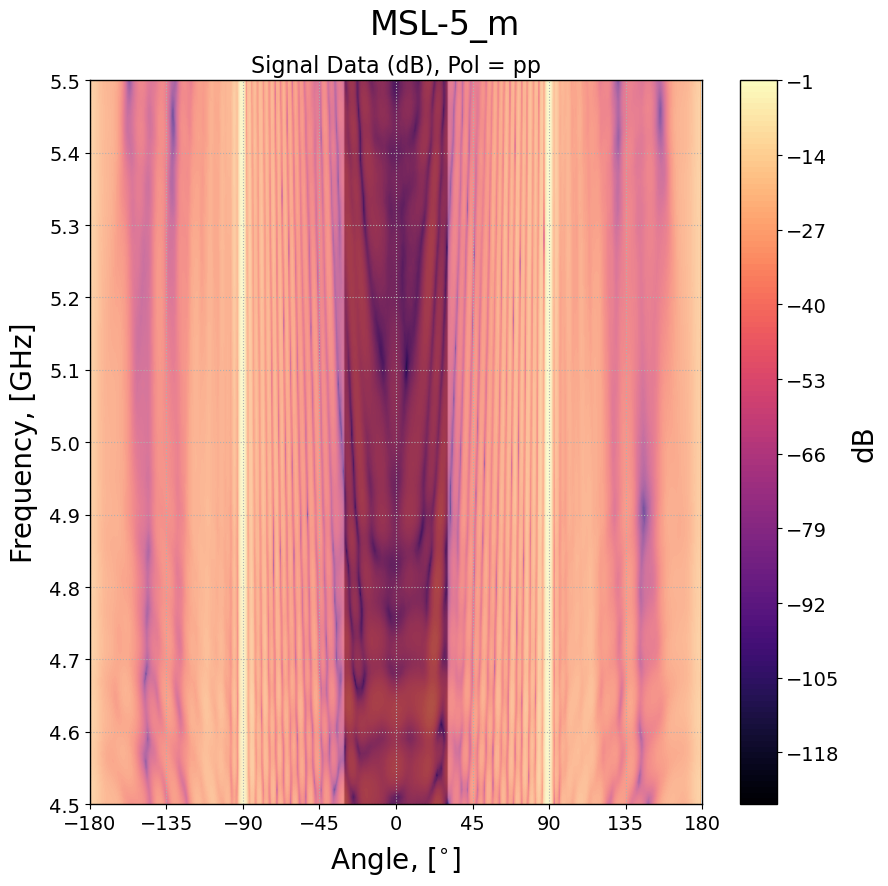
\includegraphics[width=.8\linewidth]{MSL-5_m_dB_pp.png}
    \end{subfigure}
    \caption{Missile 5 \textcolor{green}{(Test)}:  Total RCS. Vertical (tt) and Horizontal (pp) polarizations }
    \label{fig:c5}
  \end{figure}

\chapter{Simulation Results}
\label{app:simulation_results}
  \begin{figure}[htbp]
    \centering
    \begin{subfigure}{.5\textwidth}
      \centering
      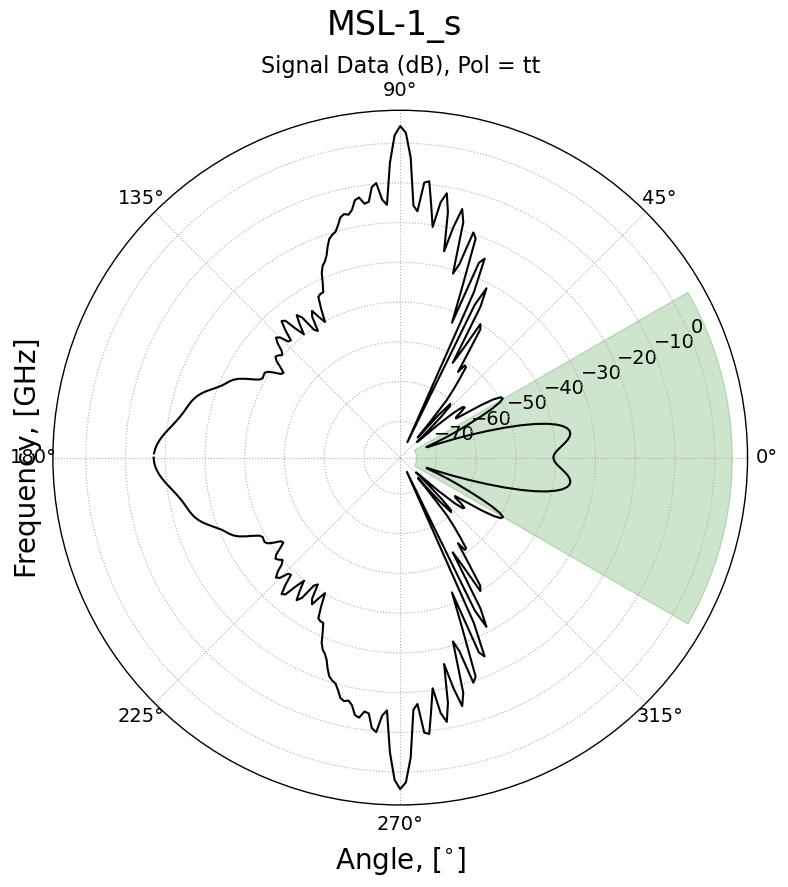
\includegraphics[width=.8\linewidth]{MSL-1_s_dB_tt_5GHz.png}
    \end{subfigure}%
    \begin{subfigure}{.5\textwidth}
      \centering
      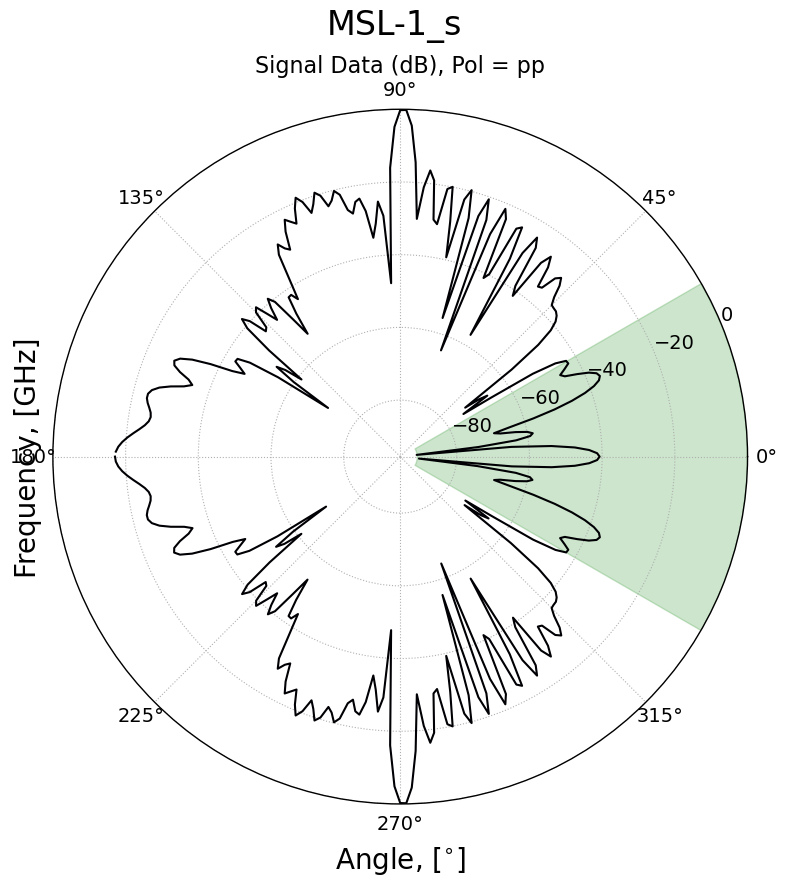
\includegraphics[width=.8\linewidth]{MSL-1_s_dB_pp_5GHz.png}
    \end{subfigure}
    \caption{Missile 1 \textcolor{red}{(Sim)}:  RCS cut at 5 GHz. Vertical (tt) and Horizontal (pp) polarizations }
    \label{fig:ns1}
  \end{figure}

  \begin{figure}[htbp]
    \centering
    \begin{subfigure}{.5\textwidth}
      \centering
      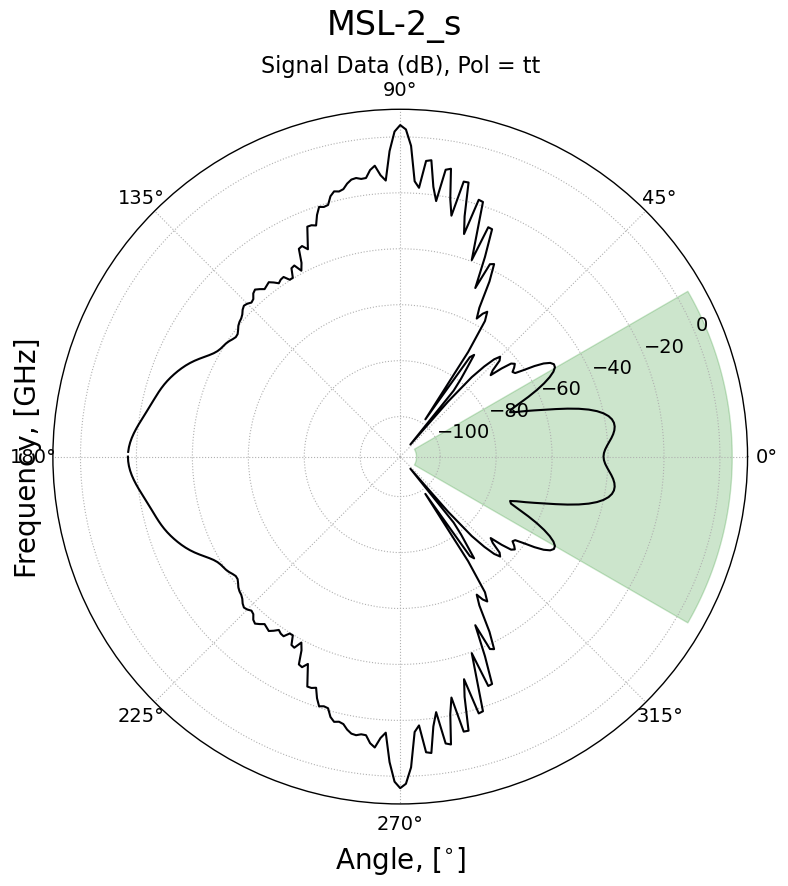
\includegraphics[width=.8\linewidth]{MSL-2_s_dB_tt_5GHz.png}
    \end{subfigure}%
    \begin{subfigure}{.5\textwidth}
      \centering
      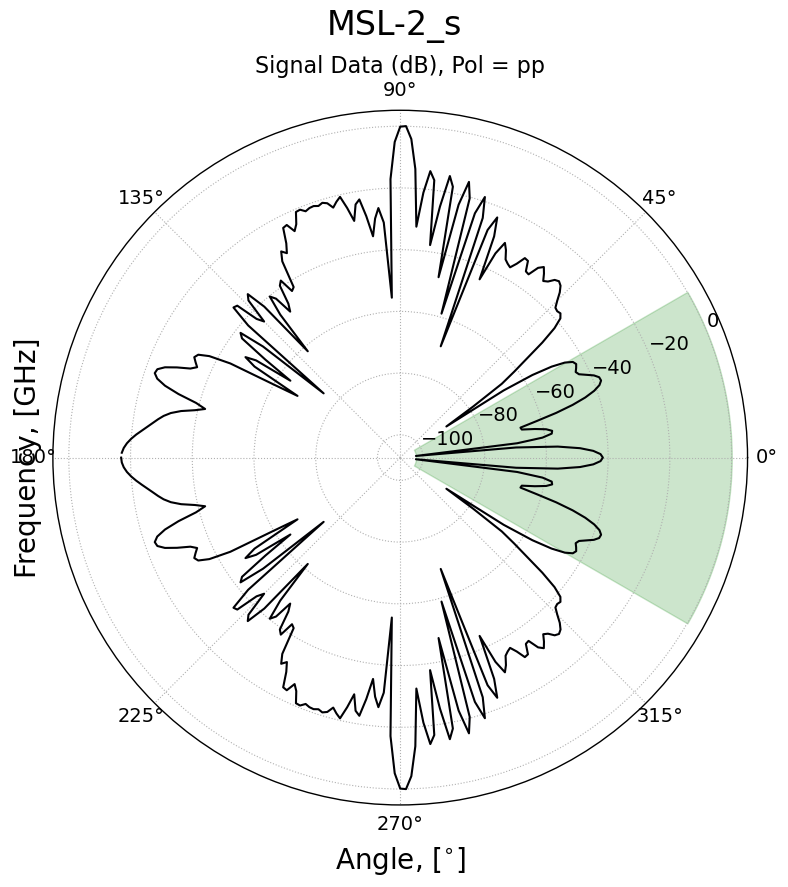
\includegraphics[width=.8\linewidth]{MSL-2_s_dB_pp_5GHz.png}
    \end{subfigure}
    \caption{Missile 2 \textcolor{red}{(Sim)}:  RCS cut at 5 GHz. Vertical (tt) and Horizontal (pp) polarizations }
    \label{fig:ns2}
  \end{figure}

  \begin{figure}[htbp]
    \centering
    \begin{subfigure}{.5\textwidth}
      \centering
      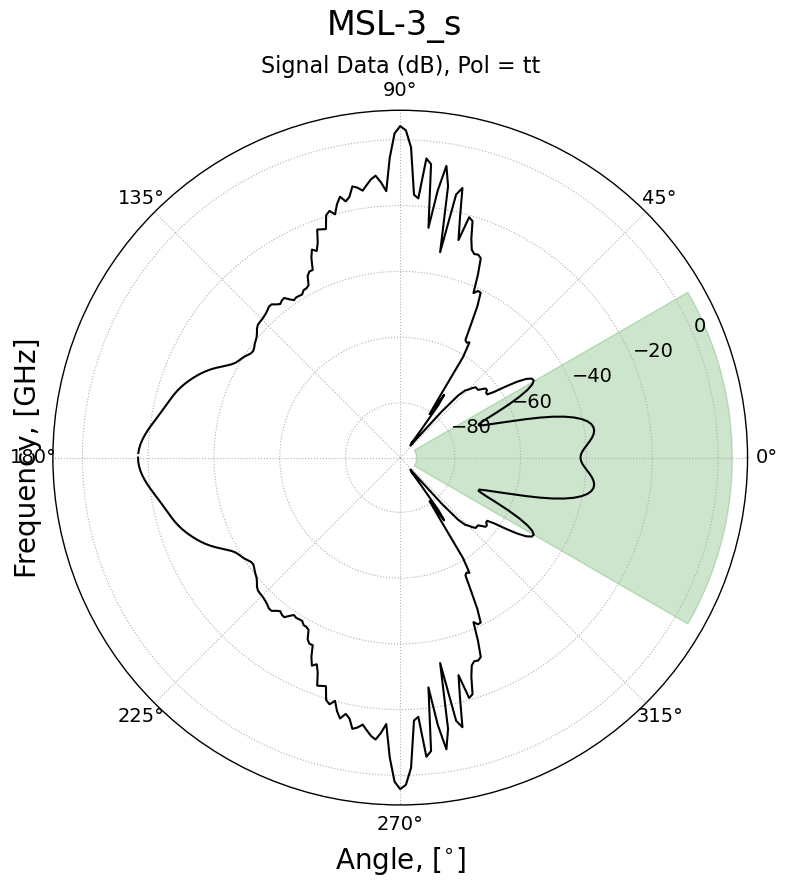
\includegraphics[width=.8\linewidth]{MSL-3_s_dB_tt_5GHz.png}
    \end{subfigure}%
    \begin{subfigure}{.5\textwidth}
      \centering
      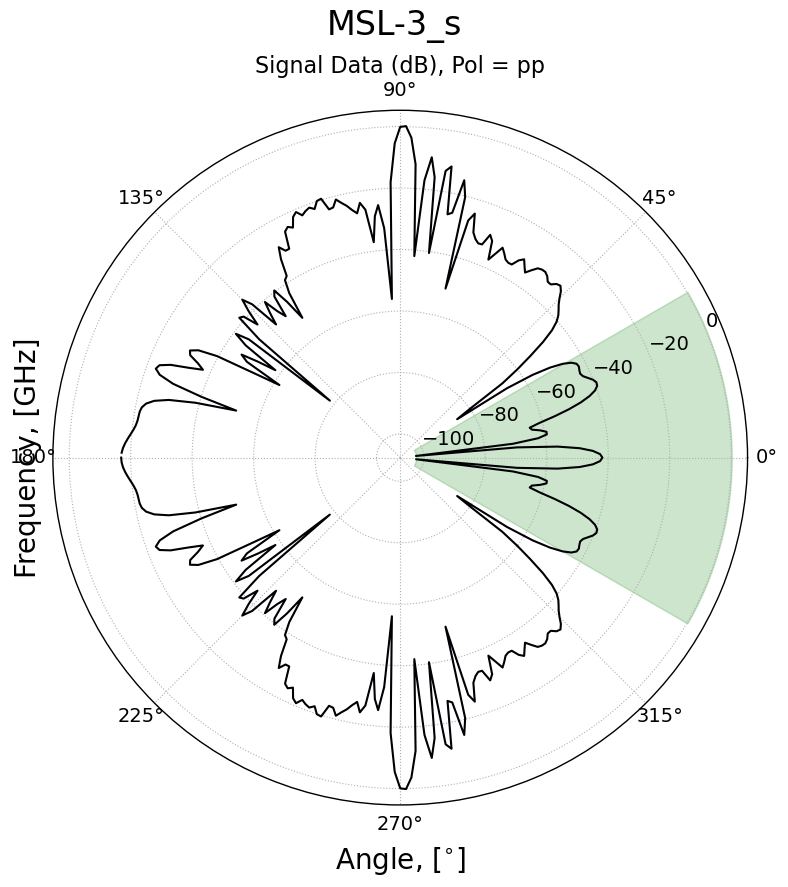
\includegraphics[width=.8\linewidth]{MSL-3_s_dB_pp_5GHz.png}
    \end{subfigure}
    \caption{Missile 3 \textcolor{red}{(Sim)}:  RCS cut at 5 GHz. Vertical (tt) and Horizontal (pp) polarizations }
    \label{fig:ns3}
  \end{figure}

  \begin{figure}[htbp]
    \centering
    \begin{subfigure}{.5\textwidth}
      \centering
      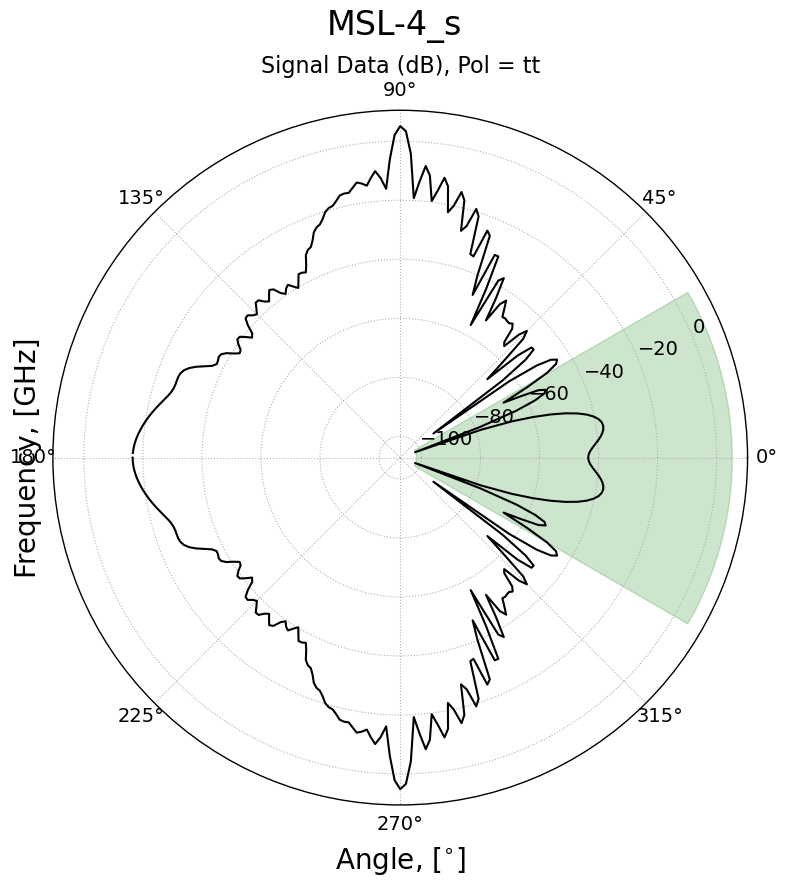
\includegraphics[width=.8\linewidth]{MSL-4_s_dB_tt_5GHz.png}
    \end{subfigure}%
    \begin{subfigure}{.5\textwidth}
      \centering
      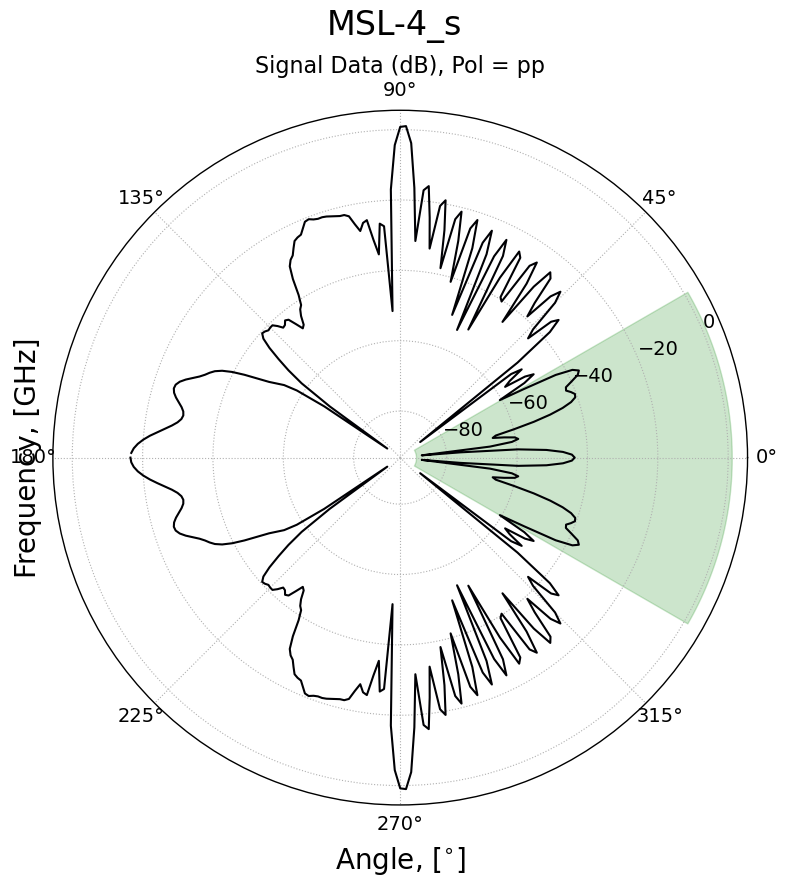
\includegraphics[width=.8\linewidth]{MSL-4_s_dB_pp_5GHz.png}
    \end{subfigure}
    \caption{Missile 4 \textcolor{red}{(Sim)}:  RCS cut at 5 GHz. Vertical (tt) and Horizontal (pp) polarizations }
    \label{fig:ns4}
  \end{figure}

  \begin{figure}[htbp]
    \centering
    \begin{subfigure}{.5\textwidth}
      \centering
      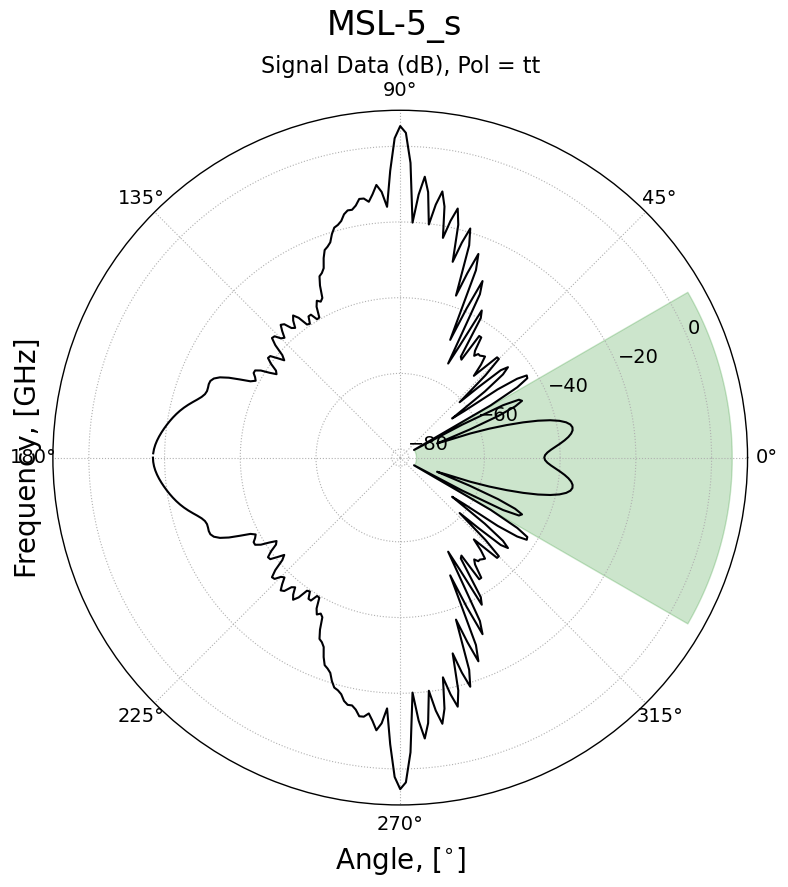
\includegraphics[width=.8\linewidth]{MSL-5_s_dB_tt_5GHz.png}
    \end{subfigure}%
    \begin{subfigure}{.5\textwidth}
      \centering
      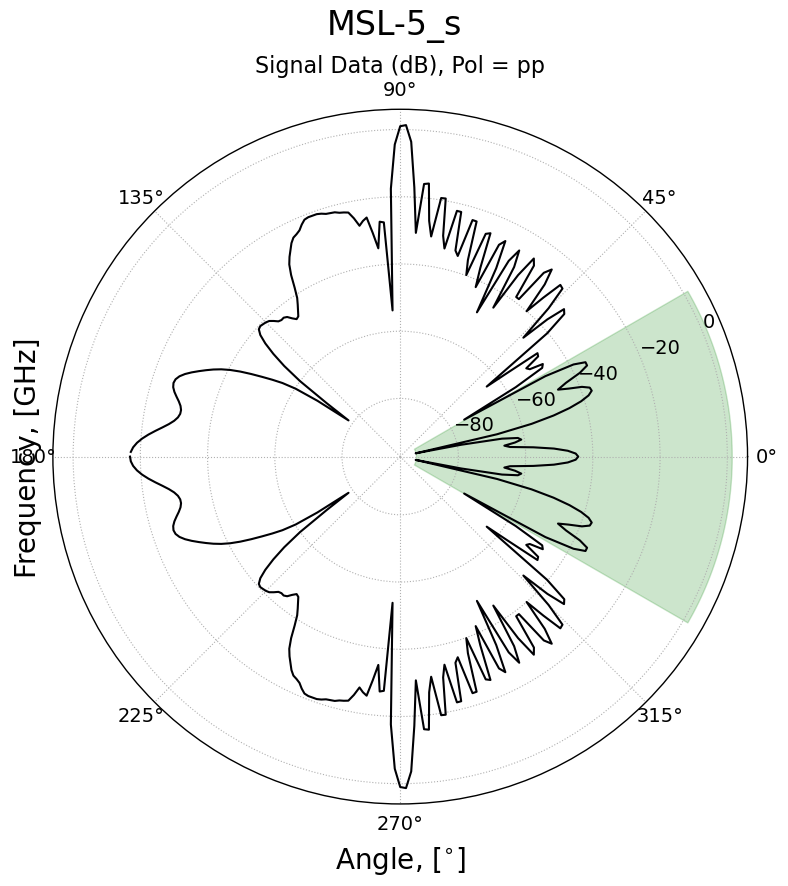
\includegraphics[width=.8\linewidth]{MSL-5_s_dB_pp_5GHz.png}
    \end{subfigure}
    \caption{Missile 5 \textcolor{red}{(Sim)}:  RCS cut at 5 GHz. Vertical (tt) and Horizontal (pp) polarizations }
    \label{fig:ns5}
  \end{figure}
